\documentclass[11pt, a4paper]{article}

% --- Packages ---
\usepackage[utf8]{inputenc}
\usepackage[T1]{fontenc}
\usepackage[margin=2.5cm]{geometry} % Page margins
\usepackage{graphicx}               % For images
\usepackage{listings}               % For including the .cfg file
\usepackage{xcolor}                 % For custom colors
\usepackage{hyperref}               % For clickable links
\usepackage{float}                  % For strict figure placement [H]
\usepackage{titlesec}
\usepackage{amsmath}                %for matrices and cases
\usepackage{amssymb}                %for special math symbols

% --- Colors and Style for the .cfg file ---
\definecolor{backcolour}{rgb}{0.95,0.95,0.96}
\definecolor{codegray}{rgb}{0.5,0.5,0.5}

\lstdefinestyle{cfgstyle}{
    backgroundcolor=\color{backcolour},   
    commentstyle=\color{codegray},
    basicstyle=\ttfamily\footnotesize,
    breakatwhitespace=false,         
    breaklines=true,                 
    captionpos=b,                    
    keepspaces=true,                 
    numbers=none,                    
    showspaces=false,                
    showstringspaces=false,
    showtabs=false,                  
    tabsize=2,
    frame=single,
    rulecolor=\color{black!30}
}

% --- Document Info ---
\title{\textbf{Multi-Agent Cooperative Defect Detection in Smart Factories}\\ \Large Distributed Autonomous Systems 2025-26}
\author{Marco Drammis, Esosa}
\date{\today}

\begin{document}

\maketitle

\tableofcontents
\vspace{1cm}
\hrule
\vspace{1cm}

\section{Distributed Classification via Logistic Regression for
Quality Control}
\subsection{Distributed Optimization}
\subsubsection{Problem Formulation}
\label{sec:problem_formulation}

The fundamental objective of the Gradient Tracking algorithm is to solve a distributed optimization problem where a network of $N$ agents aims to collaboratively minimize a global cost function. This problem is formally defined as:
\begin{equation}
    \min_z \sum_{i=1}^N \ell_i(z),
    \label{eq:global_min}
\end{equation}
where $z \in \mathbb{R}^d$ is the global decision variable and $\ell_i(z)$ represents the local cost function associated with, and known exclusively to, agent $i$. 
In our simulation framework, we assume that each agent's local cost function is a quadratic function. A general quadratic function is typically expressed as:
\begin{equation}
    \ell_i(z) = \frac{1}{2} z^\top A_i z + c_i^\top z + d_i
\end{equation}
However, in optimization problems, constant additive terms (like $d_i$) do not shift the position of the minimum (the \textit{argmin}). By completing the square and ignoring these irrelevant constant terms, any strictly convex quadratic function can be elegantly reduced to a standard, parameterized form defined solely by a matrix $Q_i$ and a vector $b_i$:

\begin{equation}
    \ell_i(z) = \frac{1}{2} (z - b_i)^\top Q_i (z - b_i)
    \label{eq:local_cost}
\end{equation}
By relying on this mathematically equivalent form, the algorithm only needs the inputs $Q_i$ and $b_i$ for each agent to seek the global consensus optimal state $z^*$.

\subsubsection*{Weight Matrix Generation}
\label{sec:topology_weights}

In a distributed optimization setting, agents communicate with each other over a network, which can be modeled as an undirected graph $\mathcal{G} = (\mathcal{V}, \mathcal{E})$. Here, $\mathcal{V} = \{1, \dots, N\}$ represents the set of agents and $\mathcal{E}$ represents the set of communication links (edges) between them. 

To ensure convergence in decentralized algorithms such as Gradient Tracking, the agents must mix their local variables using a weight matrix $W \in \mathbb{R}^{N \times N}$. This matrix must be compatible with the graph topology (i.e., $w_{ij} > 0$ only if agents $i$ and $j$ are connected, or if $i=j$) and must be doubly stochastic ($\sum_{j} w_{ij} = 1$ and $\sum_{i} w_{ij} = 1$).

A standard and highly effective method to construct such a matrix is by applying the \textbf{Metropolis-Hastings rule}. Let $\mathcal{N}_i$ be the set of neighbors of agent $i$, and let $d_i = |\mathcal{N}_i|$ be its degree (the number of neighbors it connects to). The elements $w_{ij}$ of the weight matrix $W$ are defined as follows:

\begin{equation}
    w_{ij} = 
    \begin{cases} 
    \frac{1}{\max(d_i, d_j) + 1} & \text{if } (i, j) \in \mathcal{E} \text{ and } i \neq j, \\
    1 - \sum_{k \in \mathcal{N}_i} w_{ik} & \text{if } i = j, \\
    0 & \text{otherwise.}
    \end{cases}
    \label{eq:metropolis_hastings}
\end{equation}

\subsubsection*{The Gradient Tracking Algorithm}
\label{sec:gradient_tracking}

Standard Distributed Gradient Descent (DGD) suffers from a steady-state error when using a constant step-size, as agents are pulled in different directions by their conflicting local gradients. The \textbf{Gradient Tracking} algorithm resolves this issue by introducing an auxiliary variable for each agent, $s_i^k$, which dynamically tracks the average of the global gradients across the network.

The core logic of the algorithm relies on two coupled updates occurring at each discrete iteration $k$, as shown in Figure \ref{fig:gt_formulas}.

\subsubsection*{Algorithm Initialization}
Before the iterative process begins at $k=0$, each agent $i$ must initialize its state and its gradient tracker:
\begin{itemize}
    \item \textbf{State Initialization:} $z_i^0 \in \mathbb{R}^d$. The agents can start from arbitrary initial positions in the decision space.
    \item \textbf{Tracker Initialization:} $s_i^0 = \nabla \ell_i(z_i^0)$. The gradient tracker for agent $i$ is initialized exactly to its own local gradient evaluated at the starting position $z_i^0$.
\end{itemize}

\subsubsection*{Iterative Update Rules}
At each iteration $k \geq 0$, every agent $i$ communicates with its neighbors $j \in \mathcal{N}_i$ (where the neighborhood includes the agent itself) to execute the following two steps. Note that the term $a_{ij}$ represents the mixing weights, corresponding to the elements $w_{ij}$ of the doubly stochastic matrix $W$ discussed in Section \ref{sec:topology_weights}.

\textbf{1. The State Update ($z$-update):}
\begin{equation}
    z_i^{k+1} = \sum_{j \in \mathcal{N}_i} a_{ij} z_j^k - \alpha s_i^k
    \label{eq:z_update}
\end{equation}
In this step, agent $i$ computes a weighted average of its own state and the states of its neighbors ($\sum a_{ij} z_j^k$). From this consensus state, it takes a descent step of size $\alpha$ (the learning rate). Crucially, the step is taken in the direction of the \textit{tracked global gradient} $s_i^k$, rather than its local gradient.

\textbf{2. The Tracker Update ($s$-update):}
\begin{equation}
    s_i^{k+1} = \sum_{j \in \mathcal{N}_i} a_{ij} s_j^k + \nabla \ell_i(z_i^{k+1}) - \nabla \ell_i(z_i^k)
    \label{eq:s_update}
\end{equation}
After moving to the new position $z_i^{k+1}$, agent $i$ evaluates its new local gradient $\nabla \ell_i(z_i^{k+1})$. The tracker $s_i$ is updated by taking a consensus of the neighboring trackers ($\sum a_{ij} s_j^k$) and adding the difference between its new and old local gradients. 

This specific construction ensures that, over time, every local tracker $s_i^k$ converges to the true average global gradient $\frac{1}{N} \sum_{j=1}^N \nabla \ell_j(z^k)$. As the agents approach the global minimum $z^*$, the global gradient approaches zero, allowing all agents to reach an exact consensus without steady-state oscillations.

\subsubsection{Simulation}
\label{sec:simulation_inputs}

To validate the algorithm, we established a specific test scenario (\textbf{Simulation 1}). This scenario simulates a network of $N = 3$ agents interacting over a Path Graph topology in a 3-dimensional space ($d = 3$). 

The global algorithm parameters guiding the iterative optimization process are defined as follows:
\begin{itemize}
    \item \textbf{Step-Size ($\alpha$):} $0.05$
    \item \textbf{Maximum Iterations:} $300$
    \item \textbf{Gradient Tolerance:} $10^{-4}$ (The algorithm stops early if the global gradient norm falls below this threshold).
\end{itemize}

As established in Section \ref{sec:problem_formulation}, each agent $i$ is assigned a local quadratic cost function defined by a Hessian matrix $Q_i$ and a local target vector $b_i$. Furthermore, each agent begins the simulation at a specific initial coordinate $z_i^0$. The specific configurations for the three agents are detailed below:

\subsubsection*{Agent 1}
Agent 1 aims to pull the consensus toward the origin. Its parameters are:
$$
z_1^0 = \begin{bmatrix} 10.0 \\ -5.0 \\ 2.0 \end{bmatrix}, \quad
b_1 = \begin{bmatrix} 0.0 \\ 0.0 \\ 0.0 \end{bmatrix}, \quad
Q_1 = \begin{bmatrix} 
2.00 & 0.10 & 0.00 \\ 
0.10 & 1.50 & 0.00 \\ 
0.00 & 0.00 & 1.00 
\end{bmatrix}
$$

\subsubsection*{Agent 2}
Agent 2 starts in a different region of the 3D space and targets a uniform positive coordinate:
$$
z_2^0 = \begin{bmatrix} -8.0 \\ 4.0 \\ 12.0 \end{bmatrix}, \quad
b_2 = \begin{bmatrix} 5.0 \\ 5.0 \\ 5.0 \end{bmatrix}, \quad
Q_2 = \begin{bmatrix} 
1.00 & 0.00 & 0.20 \\ 
0.00 & 2.50 & 0.00 \\ 
0.20 & 0.00 & 1.80 
\end{bmatrix}
$$

\subsubsection*{Agent 3}
Agent 3 has the strongest pull on the $X$-axis (due to the $3.00$ value in its $Q_3$ matrix) and targets a mixed-sign coordinate:
$$
z_3^0 = \begin{bmatrix} 3.0 \\ 15.0 \\ -6.0 \end{bmatrix}, \quad
b_3 = \begin{bmatrix} -5.0 \\ 2.0 \\ 8.0 \end{bmatrix}, \quad
Q_3 = \begin{bmatrix} 
3.00 & 0.20 & 0.10 \\ 
0.20 & 1.00 & 0.00 \\ 
0.10 & 0.00 & 2.00 
\end{bmatrix}
$$

These specific inputs determine the exact location of the theoretical global minimum $z^*$. During the simulation, the agents will start from their respective $z_i^0$ positions and use the weight matrix $W$ to iteratively communicate and update their states toward this shared optimal point.
\newpage

\subsubsection{Simulation Plots}
\label{sec:figures}

\begin{figure}[H]
    \centering
    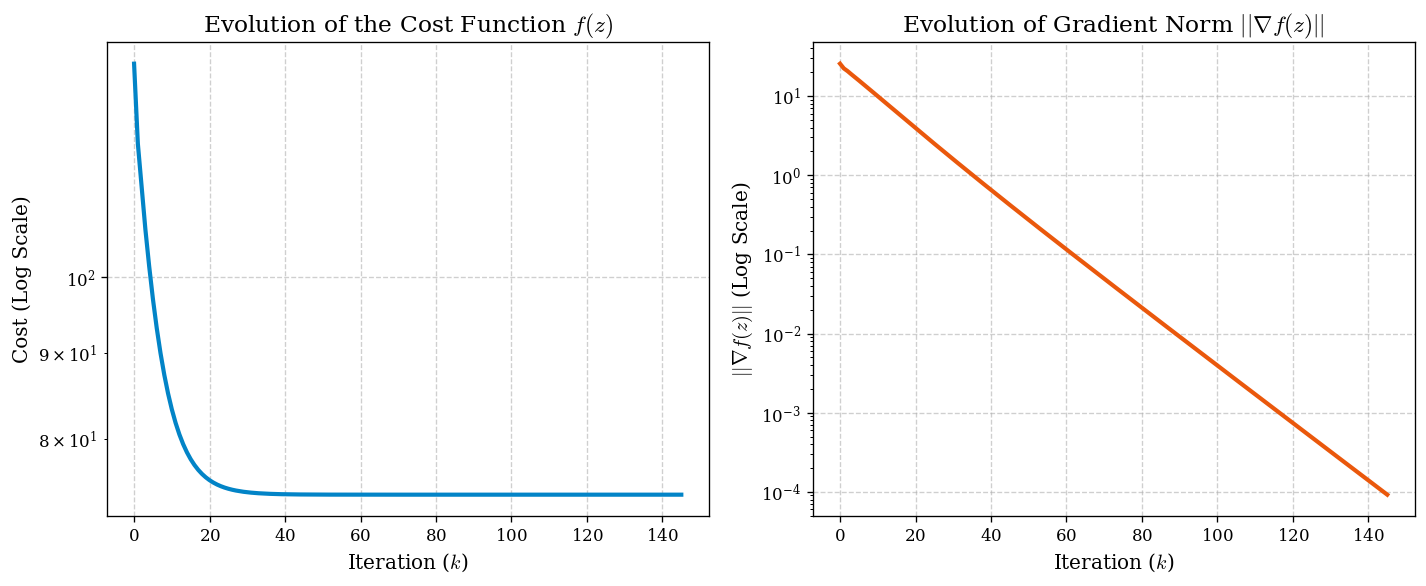
\includegraphics[width=\textwidth]{figs/gradient_tracking_simulation_1.png}
    \caption{Evolution of the Cost Function and Gradient Norm for \textbf{Simulation 1}.}
    \label{fig:sim_1}
\end{figure}

\subsubsection*{Optimization Results}

\begin{table}[h!]
\centering
\begin{tabular}{ll}
\toprule
\textbf{Metric / Parameter} & \textbf{Value} \\
\midrule
Convergence Status & \textbf{YES} (Iterations: 173/300) \\[0.5em]
Optimal Minimum ($f^*$) & $1.441138 \times 10^{2}$ \\
Final Reached Cost ($f$) & $1.441138 \times 10^{2}$ \\
Cost Error ($|f - f^*|$) & $1.038330 \times 10^{-9}$ \\[0.5em]
Theoretical Argmin ($\mathbf{z}^*$) & $[3.3627,\, 2.1153,\, 0.9723]^\top$ \\
Final Reached Argmin ($\mathbf{z}$) & $[3.3626,\, 2.1153,\, 0.9723]^\top$ \\
Position Error ($\|\mathbf{z} - \mathbf{z}^*\|$) & $2.221832 \times 10^{-5}$ \\
\bottomrule
\end{tabular}
\end{table}


\end{document}